\section{Проектирование программного средства}

\subsection{Разработка архитектуры программного средства}

После того, как были сформулированы функциональные требования к разрабатываемой
системе,  а  также  исходя  из  результатов  анализа  существующих
программных решений, можно определить основные моменты организации системы,  в
которой  будет  функционировать  разрабатываемое  программное  решение.

Процесс проектирования архитектуры программного обеспечения включает в себя сбор
требований, их анализ и создание проекта для компонента программного
обеспечения в соответствие с требованиями. Успешная разработка ПО должна
обеспечивать баланс неизбежных компромиссов вследствие противоречащих
требований;  соответствовать  принципам  проектирования  и  рекомендованным
методам,  выработанным  со  временем;  и  дополнять  современное оборудование,
сети и системы управления. 

Архитектуру  программного  обеспечения  можно рассматривать  как  сопоставление
между целью компонента ПО и сведениями о реализации в коде. Правильное понимание
архитектуры  обеспечит  оптимальный баланс требований и результатов. Только
программное обеспечение с хорошо продуманной архитектурой способно выполнять
указанные задачи с параметрами исходных требований, одновременно обеспечивая
максимально высокую производительность. Программное средство построено на основе
модульной архитектуры. 

\FloatBarrier
\begin{figure}[H]
\centering
	\fbox{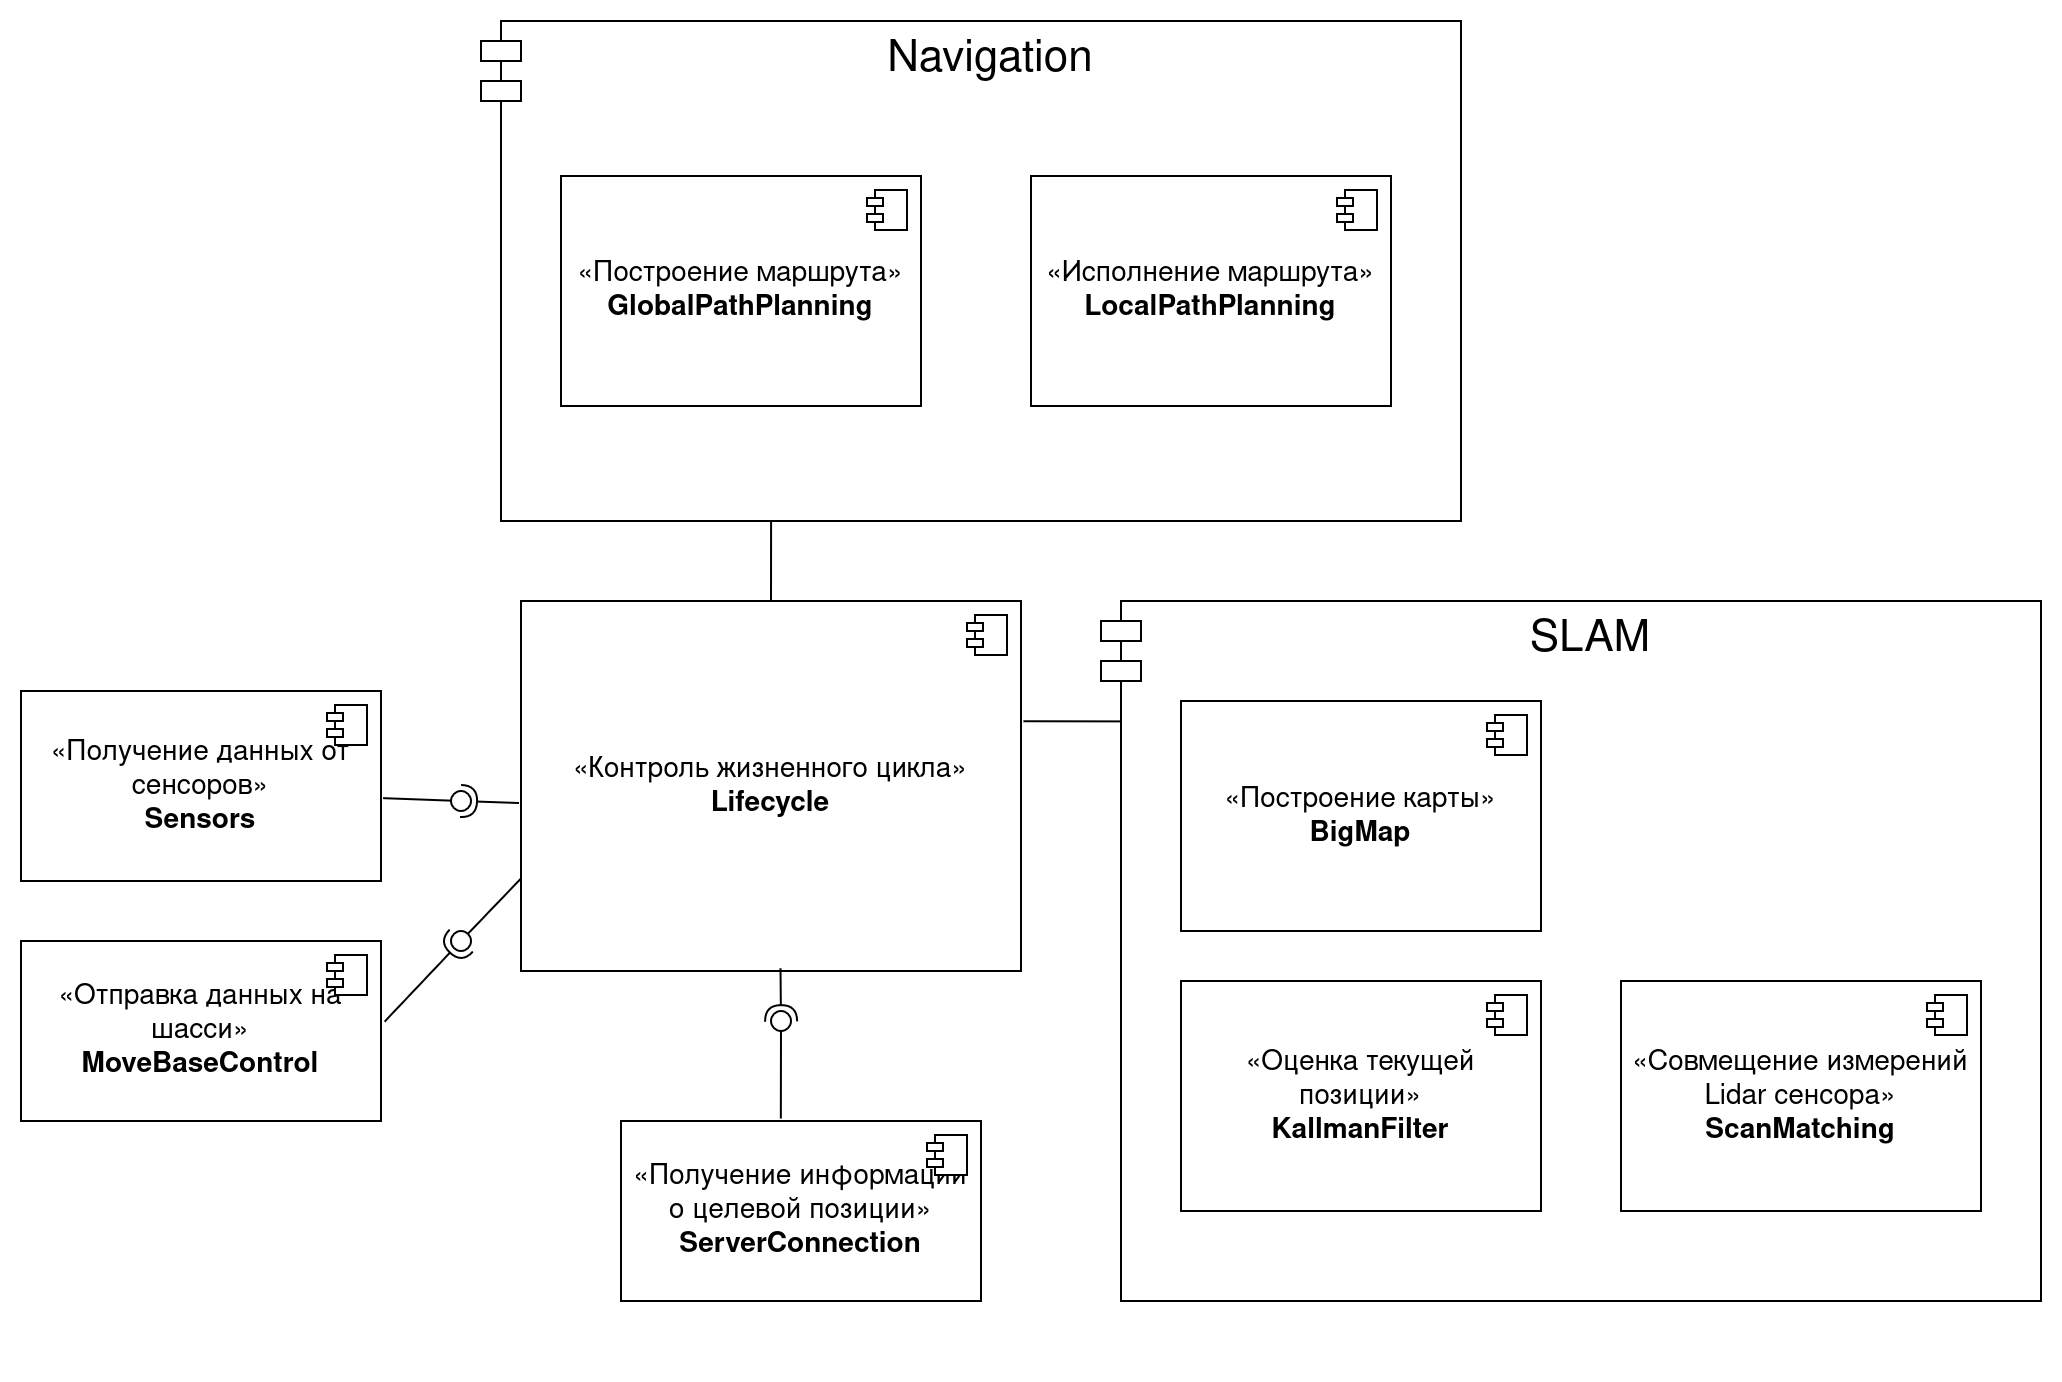
\includegraphics[width=11cm]{MODULES.drawio}}
\caption{Диаграмма компонентов проектируемого ПО}
\label{fig:components}
\end{figure}

На рисунке \ref{fig:components} отображены модули системы:~
\begin{itemize}
	\item модуль жизненного цикла;
	\item модуль построения маршрута;
	\item модуль исполнения маршрута;
	\item модуль получения данных сенсоров;
	\item модуль отправки данных на шасси;
	\item модуль получения информации о целевой позиции;
	\item модуль построения карты;
	\item модуль оценки позиции;
	\item модуль совмещения измерений LIDAR сенсора.
\end{itemize}

% \todo{Общая схема программы}
Коммуникация между модулями осуществляется через модуль жизненного цикла, все
модули получают и отправляют информацию через него, не считая сильно-связных
модулей в системе SLAM. 

% Модули сбора информации
Модуль получения данных сенсоров осуществляет сбор информации: 2D LIDAR
предоставляет информацию о расстояниях до объектов в окружающем пространстве,
IMU -- об угловых ускорениях и наклоне устройства, а GPS -- о
глобальном местоположении. Все эти данные передаются в модуль SLAM, который
использует их для построения карты окружающей среды и вычисления текущего
местоположения робота. Это позволяет системе иметь точную картину окружающего
мира и следить за положением устройства.

Модуль совмещения измерений LIDAR сенсора, является основой для построения карты
и локализации робота. С помощью данных от лидаров и модуля оценки позиции он
строит карту пространства, постоянно обновляя ее по мере движения робота, и
вычисляет его местоположение относительно этой карты. Это позволяет системе
динамично корректировать действия робота в зависимости от изменений в окружающей
среде, таких как появление новых препятствий или изменение положения объектов.

Полученные от совмещения измерений данные о местоположении робота передаются в модуль оценки
позиции. Этот модуль анализирует текущее положение устройства с использованием
фильтрации и различных методов оценки, таких как фильтр Калмана. Оценка позиции
робота имеет важное значение для корректного планирования маршрута, поскольку
точность информации о местоположении напрямую влияет на точность движений
устройства.

Модуль создания маршрута отвечает за вычисление оптимального пути от текущего
местоположения робота до заданной цели. Этот модуль использует данные о
местоположении, а также информацию о препятствиях, чтобы планировать наиболее
эффективный и безопасный маршрут. Важно, чтобы система могла адаптироваться к
изменениям окружающей среды, например, при возникновении новых препятствий,
система должна пересчитать маршрут в реальном времени, обеспечивая продолжение
движения робота без ошибок.

После того как маршрут спланирован, информация о нем передается в модуль
управления моторами. Этот модуль отвечает за выполнение команд, таких как
движение вперед, повороты и торможение. Модуль управления моторами должен
обеспечить точное выполнение команд с минимальными задержками, чтобы робот мог
двигаться по маршруту с высокой точностью. Кроме того, он должен поддерживать
оперативную реакцию на данные от сенсоров, такие как сигнал от лидаров,
предупреждающий о близко расположенных препятствиях.

При обнаружении препятствий вблизи, например, если расстояние до объекта
становится меньше заданного порога, система должна немедленно реагировать. Это
может быть реализовано командой «стоп», которая отправляется в модуль управления
моторами для немедленной остановки робота. Такие меры безопасности необходимы
для предотвращения столкновений и обеспечения безопасной работы робота в
различных условиях.


\subsection{Алгоритмы фильтрации}
Используя сенсоры можно получать информацию о текущей позиции и скорости робота.
Сенсоры выдают значения с определённой погрешностью, из-за чего прямое
использование их значений приводит к неточной оценки позиции.

С помощью алгоритмов фильтрации несколько показаний с погрешностью сенсоров
можно комбинировать между собой и получать более точное приближение состояния.
Обычно в качестве состояния используется текущая позиция и ускорение.

Существует большое количество алгоритмов, позволяющие решать задачу оценки
состояния c учётом заданных ограничений (например, ограничений по доступным
вычислительным мощностям):

\begin{itemize}
	\item линейный фильтр Калмана (см. пункт $\ref{kf}$);
	\item расширенный фильтр Калмана (см. пункт $\ref{ekf}$);
	\item нелинейный фильтр Калмана (см. пункт $\ref{sec:ukf_info}$);
\end{itemize}

Каждый метод анализируется с точки зрения его математической основы и
применимости в задачах навигации.

\subsubsection{Фильтр Калмана}
\label{kf}
Фильтр Калмана -- рекурсивный алгоритм, обеспечивающий оптимальную оценку
состояния линейной динамической системы с нормально распределёнными шумами.
Предположение, что шум системы нормально распределён является ключевым. Динамику
системы в момент времени \( k \) можно описывается уравнением момент времени:
\begin{align}
    \mathbf{x}_k &= \mathbf{F}_k \mathbf{x}_{k-1} + \mathbf{B}_k \mathbf{u}_k + \mathbf{w}_k, \label{eq:kalman_state} \\
    \mathbf{z}_k &= \mathbf{H}_k \mathbf{x}_k + \mathbf{v}_k. \label{eq:kalman_meas}
\end{align}

\begin{explanationx}
	\item[где] \(\mathbf{x}_k\) -- вектор переменных состояния;
	\item \(\mathbf{z}_k\) -- вектор переменных измерений;
	\item \(\mathbf{u}_k\) -- управляющие переменные;
	\item \(\mathbf{w}_k\) шум процесса;
	\item \(\mathbf{v}_k \) -- шум измерений;
	\item \(\mathbf{F}_k\) -- матрица перехода состояния;
	\item \(\mathbf{B}_k\) -- матрица управления;
	\item \(\mathbf{H}_k\) -- матрица измерений.
\end{explanationx}

Переменные состояния (\(\mathbf{x}_k\)) описывают характеристики системы на временном шаге \( k \).
Переменные состояния полностью определяют её динамическое поведение.
Переменные измерения (\(\mathbf{z}_k\)) представляют наблюдаемые данные, получаемые от датчиков на шаге \( k \). 
Они описываются моделью измерений (см. уравнение \ref{eq:kalman_meas})
Управляющие переменные (\(\mathbf{u}_k\)) описывают внешние воздействия на систему, влияющие на её динамику.
Они входят в уравнение состояния и считаются известными, предоставляемыми системой управления.
Например, команды управления для перемещающегося средства.

Матрица перехода состояния \(\mathbf{F}_k\) описывает эволюцию состояния системы \(\mathbf{x}_k\) во времени без учёта управления и шума.
Матрица управления \(\mathbf{B}_k\) описывает влияние управляющего сигнала \(\mathbf{u}_k\) на состояние системы. Она также входит в уравнение состояния и имеет размер \(n \times m\), где \(m\) -- размерность \(\mathbf{u}_k\).

В идеальных условиях, шум процесса \(\mathbf{w}_k\) и шум измерений \(\mathbf{м}_k\)
полагаются равны 0. Шум процесса устанавливается в зависимости от степени
доверия системе и измерениям.

Все переменные, в зависимости от возможности произвести наблюдение за значением,
можно разделить на скрытые и явные зависимости.
К скрытым переменным относят:
\begin{itemize}
    \item переменные состояния $\mathbf{x}_k$; 
    \item шум процесса $\mathbf{w}_k$.
\end{itemize}

К явным переменным относят:
\begin{itemize}
    \item переменные измерений $\mathbf{z}_k$; 
    \item управляющие переменные $\mathbf{u}_k$; 
    \item шум измерений $\mathbf{v}_k$.
\end{itemize}

Работа фильтра Калмана основана на последовательном выполнении этапов предсказания (predict) и 
коррекции (update).

На этапе предсказания выполняется расчёт 
априорной оценки переменных состояния (см. уравнение \ref{x_predict})
и априорной оценки ковариация ошибка системы (см. уравнение \ref{p_predict}).
\begin{align}
\hat{\mathbf{x}}_{k|k-1} &= \mathbf{F}_k \hat{\mathbf{x}}_{k-1|k-1} + \mathbf{B}_k \mathbf{u}_k, \label{x_predict}\\
\mathbf{P}_{k|k-1} &= \mathbf{F}_k \mathbf{P}_{k-1|k-1} \mathbf{F}_k^T + \mathbf{Q}_k. \label{p_predict}.
\end{align}

Этап коррекции обновляет априорную оценку с учётом измерений, полученных с использованием датчиков.
Для этого вычисляются коэффициент усиления Калмана \(\mathbf(K)_k\) (см. уравнение \ref{kf_gain}),
апостериорная оценка состояния \(\mathbf{x}_{k|k}\) (см. уравнение \ref{x_update}),
и апостериорная ковариация ошибки \(\mathbf{P}_{k|k}\) (см. уравнение \ref{p_update}).

\begin{equation}
\label{kf_gain}
\mathbf{K}_k = \mathbf{P}_{k|k-1} \mathbf{H}_k^T (\mathbf{H}_k \mathbf{P}_{k|k-1} \mathbf{H}_k^T + \mathbf{R}_k)^{-1},
\end{equation}

\begin{equation}
\label{x_update}
\hat{\mathbf{x}}_{k|k} = \hat{\mathbf{x}}_{k|k-1} + \mathbf{K}_k (\mathbf{z}_k - \mathbf{H}_k \hat{\mathbf{x}}_{k|k-1}),
\end{equation}

\begin{equation}
\label{p_update}
\mathbf{P}_{k|k} = (\mathbf{E} - \mathbf{K}_k \mathbf{H}_k) \mathbf{P}_{k|k-1}.
\end{equation}
\\

Коэффициент \(\mathbf{K}_k\) балансирует доверие к модели и измерениям, снижая неопределённость.

\subsubsection{Расширенный фильтр Калмана (Extended Kalman Filter)}
\label{ekf}


Расширенный фильтр Калмана (EKF) адаптирует фильтр Калмана (KF) для нелинейных систем:

\begin{align}
    \mathbf{x}_k &= \mathbf{f}(\mathbf{x}_{k-1}, \mathbf{u}_k) + \mathbf{w}_k, \\
    \mathbf{z}_k &= \mathbf{h}(\mathbf{x}_k) + \mathbf{v}_k.
\end{align}

Линеаризация выполняется с помощью матриц Якоби \(\mathbf{F}_k = \frac{\partial \mathbf{f}}{\partial \mathbf{x}}\big|_{\hat{\mathbf{x}}_{k-1|k-1}}\) и \(\mathbf{H}_k = \frac{\partial \mathbf{h}}{\partial \mathbf{x}}\big|_{\hat{\mathbf{x}}_{k|k-1}}\). Этапы предсказания и коррекции аналогичны фильтру Калмана, но ошибки линеаризации снижают точность при сильной нелинейности.

\subsubsection{Нелинейный фильтр Калмана (Unscented Kalman Filter)}
\label{sec:ukf_info}

UKF использует сигма-точки для обработки нелинейностей без линеаризации. Сигма-точки генерируются на основе \(\hat{\mathbf{x}}_{k-1|k-1}\) и \(\mathbf{P}_{k-1|k-1}\), затем распространяются через \(\mathbf{f}\) и \(\mathbf{h}\):
\begin{align}
    \hat{\mathbf{x}}_{k|k-1} &= \sum w_i \mathbf{f}(\mathbf{x}_i), \\
    \mathbf{P}_{k|k-1} &= \sum w_i (\mathbf{f}(\mathbf{x}_i) - \hat{\mathbf{x}}_{k|k-1})(\mathbf{f}(\mathbf{x}_i) - \hat{\mathbf{x}}_{k|k-1})^T + \mathbf{Q}_k.
\end{align}
Для состояния \(\mathbf{x}_{k-1|k-1}\) с оценкой 
\(\hat{\mathbf{x}}_{k-1|k-1}\) и ковариацией \(\mathbf{P}_{k-1|k-1}\) 
генерируется \(2n + 1\) сигма-точек, где \(n\)  -- это размерность вектора состояний \(\mathbf{x}_k\).
Для генерации точек используется следующий алгоритм:

\begin{itemize}
    \item вычисление масштабирующего параметра:
    \[
    \lambda = \alpha^2 (n + \kappa) - n,
    \]
    где \(\alpha\) (\(10^{-3} \leq \alpha \leq 1\)) контролирует разброс, \(\kappa\) (обычно \(3 - n\)) -- параметр настройки.
    \item генерация сигма-точек:
    \[
    \mathbf{x}_{k-1}^{(0)} = \hat{\mathbf{x}}_{k-1|k-1},
    \]
    \[
    \mathbf{x}_{k-1}^{(i)} = \hat{\mathbf{x}}_{k-1|k-1} + (\sqrt{(n + \lambda) \mathbf{P}_{k-1|k-1}})_i, \quad i = 1, \dots, n,
    \]
    \[
    \mathbf{x}_{k-1}^{(i)} = \hat{\mathbf{x}}_{k-1|k-1} - (\sqrt{(n + \lambda) \mathbf{P}_{k-1|k-1}})_{i-n}, \quad i = n+1, \dots, 2n,
    \]
    где \((\sqrt{(n + \lambda) \mathbf{P}_{k-1|k-1}})_i\) -- \(i\)-й столбец разложения Холецкого.
    \item назначение весов:
    \[
    w_m^{(0)} = \frac{\lambda}{n + \lambda}, \quad w_m^{(i)} = \frac{1}{2(n + \lambda)}, \quad i = 1, \dots, 2n,
    \]
    \[
    w_c^{(0)} = \frac{\lambda}{n + \lambda} + (1 - \alpha^2 + \beta), \quad w_c^{(i)} = \frac{1}{2(n + \lambda)}, \quad i = 1, \dots, 2n,
    \]
    где \(\beta \approx 2\) для нормального распределения.
\end{itemize}

В общем случае, UKF работает более точно, чем EKF:
\begin{itemize}
    \item высокая точность при сильной нелинейности, так как сигма-точки лучше аппроксимируют распределение;
    \item отсутствие необходимости вычислять производные, что упрощает реализацию для сложных функций.
\end{itemize}

\subsection{AHRS}
\label{subsec:ahrs}

Система ориентации и курса (Attitude and Heading Reference System или AHRS) предназначена для оценки
ориентации объекта: углов крена (roll), тангажа (pitch) и рысканья (yaw).
В задачах навигации, подобных тем, где применяются фильтр частиц (PF) или фильтры Калмана,
AHRS играет ключевую роль в определении ориентации.
Основные источники данных, для которых используется AHRS: 
\begin{itemize}
    \item гироскопы (\(\boldsymbol{\omega} = [\omega_x, \omega_y, \omega_z]^T\)) для измерения угловой скорости;
    \item акселерометры (\(\mathbf{a} = [a_x, a_y, a_z]^T\)) для оценки крена и тангажа через вектор силы тяжести;
    \item магнитометры (\(\mathbf{m} = [m_x, m_y, m_z]^T\)) для определения рысканья относительно магнитного севера.
\end{itemize}

Ориентация представляется в системе кватернионом \(\mathbf{q} = [q_0, q_1, q_2, q_3]^T\), что позволяет
избежать блокировки кардана (gimbal lock).

Применение AHRS ограничивается рядом внешних условий:

\begin{enumerate}[label=\arabic*]
    \item Наличие магнитных помех искажают показания магнитометров.
    \item Дрейф гироскопов требует внешней коррекции. Использование алгоритмов фильтрации
	    с AHRS позволяет произвести корректировку дрейфа гироскопов.
    \item AHRS не моделирует положение и линейную скорость.
\end{enumerate}

\subsection{Оценка измерений в AHRS}

Для оценки ориентации в AHRS принято использовать один из двух алгоритмов: фильтр Маджвика или фильтр Махони.

\subsubsection{Фильтр Маджвика}

Фильтр Маджвика использует градиентный спуск для минимизации ошибки гироскопа 
с коррекцией от акселерометра и магнитометра. Он оценивает кватернион ориентации
\(\mathbf{q}_t\) путём численного интегрирования:

\begin{equation}
    \dot{\mathbf{q}}_t = \dot{\mathbf{q}}_{\omega, t} - \beta \dot{\mathbf{q}}_{\epsilon, t},
\end{equation}

\begin{explanationx}
\item[где] \(\dot{\mathbf{q}}_{\omega, t} = \frac{1}{2} \mathbf{q}_{t-1} \otimes \begin{bmatrix} 0 \\ 
\boldsymbol{\omega}_t \end{bmatrix}\) -- изменения ориентации от гироскопа \(\boldsymbol{\omega}_t\);
\item \(\dot{\mathbf{q}}_{\epsilon, t}\) -- 
	численное значение ошибки, вычисленное градиентным спуском из данных акселерометра 
	(\(\mathbf{a}_t\)) и магнитометра (\(\mathbf{m}_t\));
\item \(\beta\) -- коэффициент доверия к фильтру ($\beta \in [0.1, 1]$).
\end{explanationx}

Основными преимуществами фильтра Маджвика являются:
\begin{itemize}
	\item высокая точность вычисления ориентации;
	\item эффективная компенсация дрейфа гироскопа.
\end{itemize}

\subsubsection{Фильтр Махони}

Фильтр Махони основан на нелинейном комплементарном фильтре на группе \(SO(3)\).
Он минимизирует ошибку между измеренными и эталонными векторами с помощью пропорционально-интегрального (PI)
компенсатора. Ориентация обновляется как:

\begin{equation}
 \dot{\mathbf{q}}_t = \frac{1}{2} \mathbf{q}_t \otimes \begin{bmatrix} 0 \\ \boldsymbol{\omega}_t + \mathbf{e}_t \end{bmatrix},
\end{equation}
\begin{explanationx}
\item[где]
    \(\mathbf{e}_t = k_P \boldsymbol{\omega}_{\text{err}} + k_I \int \boldsymbol{\omega}_{\text{err}} \, dt\) --
    коррекция, основанная на ошибке \(\boldsymbol{\omega}_{\text{err}}\), 
    вычисленной как векторное произведение измеренных и предсказанных векторов.
    \(k_P \approx 1\), \(k_I \approx 0.3\) -- PI-компенсатора.
\end{explanationx}

К основным преимуществам фильтра Махони относят:
\begin{itemize}
	\item быстрая сходимость;
	\item низкая вычислительная сложность.
\end{itemize}

Фильтр требует тщательного выбора параметров \(k_P\), \(k_I\). По сравнению с фильтром Маджвика, 
фильтр Махони хуже оценивает ориентацию в пространстве.


Таким образом, оба фильтра имеют место быть для различных условий применения.
Фильтр Маджвика предоставляет большую точность на низкой частоте отправке данных.
Фильтр Махони используются на системах с ограниченной вычислительной мощностью.

% \subsection{Алгоритмы SLAM}
% В подразделе \ref{sec:ros_analysys} шла речь о двух основных типов алгоритмов.
% Более ранние алгоритмы, основанные на фильтрах Байеса, и более новые методы,
% основанные на графах.
% Рассмотрим сначала подходы основанные на фильтрах Байеса.
%
% \subsubsection{Фильтры байеса}
% % NN generated
%
% \subsubsection{SLAM основанный на графах}

\subsection{Сетка занятости (Occupancy grid)}

Карта занятости (Occupancy Grid) в двумерном представлении является сеткой,
разделяющей пространство на регулярные ячейки, каждая из которых отражает
состояние окружающей среды. Каждая ячейка хранит информацию о вероятности
наличия препятствия, принимая значения, соответствующие состояниям: занята
(препятствие присутствует), свободна (доступно для движения) или неизвестна
(данные отсутствуют). Карты формируются на основе данных сенсоров, и обновляются
в реальном времени, позволяя роботу адаптироваться к динамическим изменениям в
среде.

Двумерные карты занятости широко применяются в мобильной робототехнике для задач
навигации и планирования маршрутов. Они обеспечивают простое и эффективное
представление окружающей среды, позволяя роботу определять свободные пути,
избегать препятствий и строить оптимальные траектории движения. Благодаря своей
структуре, такие карты легко интегрируются в алгоритмы локализации и
картирования (SLAM), что делает их ключевым инструментом для автономного
передвижения мобильных роботов в сложных условиях.

\subsection{Построение карты}

\subsubsection{ICP}
Iterative Closest Point (ICP) -- классический алгоритм регистрации облаков
точек, широко используемый в компьютерном зрении и робототехнике для точного
выравнивания двух наборов данных, полученных с помощью лидаров или других
3D-сканеров.

Основная цель ICP -- расстояние между двумя облаками точек:
фиксированным эталонным (reference) и подвижным (source), который необходимо
трансформировать (сдвинуть и повернуть) так, чтобы максимально приблизить к
эталону. Алгоритм работает итеративно, последовательно уточняя параметры
преобразования.

1 Алгоритм начинается с предварительной оценки преобразования, которое
приблизительно совмещает исходное облако с эталонным. Качество начального
приближения существенно влияет на результат, поскольку ICP может сойтись к
локальному минимуму.
    
2 Для каждой точки подвижного облака находится ближайшая точка в эталонном
облаке по евклидову расстоянию. Для ускорения поиска обычно используется
структура данных k-d дерево.
    
3 На основе найденных пар точек вычисляется оптимальное преобразование (смещение
и поворот), минимизирующее среднеквадратичное расстояние между соответствующими
точками. Часто применяется метод наименьших квадратов.
    
4 Подвижное облако точек трансформируется с использованием найденного
преобразования.
    
5 Шаги поиска соответствий и оценки преобразования повторяются до тех пор, пока
изменение ошибки не станет меньше заданного порога или не будет достигнуто
максимальное число итераций.

\subsubsection{Особенности и ограничения ICP}
\begin{itemize}
	\item ICP чувствителен к качеству начального приближения и может застревать
		в локальных оптимумах;
	\item алгоритм хорошо работает при небольших смещениях и поворотах между
		сканами;
	\item существует множество вариантов ICP, включая point-to-point (точка к
		точке) и point-to-plane (точка к плоскости), последний из которых лучше
		подходит для структурированных поверхностей;
\end{itemize}

ICP является базовым инструментом для регистрации 2D и 3D данных в задачах SLAM,
реконструкции объектов и навигации мобильных платформ, особенно когда требуется
точное совмещение облаков точек, полученных с разных позиций или в разное время.

Таким образом, ICP -- эффективный и относительно простой алгоритм,
обеспечивающий точное выравнивание облаков точек за счёт итеративного уточнения
преобразования между ними.

В алгоритме Iterative Closest Point (ICP) задача сводится к поиску оптимального
жёсткого преобразования (поворота и сдвига), которое минимизирует сумму
квадратов расстояний между соответствующими точками двух облаков. Для решения
этой задачи на каждом шаге, когда соответствия между точками уже известны,
широко применяется метод сингулярного разложения матриц (SVD, Singular Value
Decomposition).

\subsection{Построение маршрута}
Глобальные планировщики предназначены для построения маршрута от начальной точки
до цели в известной или частично известной среде, обычно представленной в виде
графа или сетки. В качестве глобальных планировщиков используют:
\begin{itemize}
	\item алгоритм Дейкстры;
	\item алгоритм A*;
	\item алгоритм RRT.
\end{itemize}

\subsubsection{Алгоритм Дейкстры}

Алгоритм Дейкстры служит для поиска кратчайшего пути в графе с неотрицательными
весами рёбер. Начиная с начальной вершины, алгоритм последовательно обновляет
расстояния до всех остальных вершин, выбирая на каждом шаге вершину с
минимальным текущим расстоянием. Для выбранной вершины проверяются её соседи, и
расстояния до них обновляются, если найден более короткий путь. Процесс
продолжается до обработки всех вершин или достижения цели.

Математически алгоритм минимизирует расстояние до вершины $v$ по формуле:

\begin{equation}
d[v] = \min_{u \in V} \{ d[u] + w(u, v) \},
\end{equation}

\begin{explanationx}
\item[где] $d[v]$ -- кратчайшее расстояние от начальной вершины до $v$;
\item $w(u, v)$ -- вес ребра между вершинами $u$ и $v$.
\end{explanationx}

Алгоритм гарантирует оптимальность пути,
но для больших графов требует значительных вычислений,
с временной сложностью $O((V + E) \log V)$ при использовании кучи.

\subsubsection{Алгоритм A*}
Алгоритм A* улучшает подход Дейкстры,
добавляя эвристическую функцию для ускорения поиска.
Каждая вершина оценивается по сумме стоимости пути от начальной точки ($g(v)$)
и эвристической оценки расстояния до цели ($h(v)$).
Выбирается вершина с минимальной суммой $f(v) = g(v) + h(v)$.
Эвристика должна быть допустимой, то есть не переоценивать истинное расстояние: $h(v) \leq h^*(v)$,
где $h^*(v)$ -- реальное расстояние до цели.

Логику алгоритма можно описать формулой:
\begin{equation}
f(v) = g(v) + h(v).
\end{equation}

A* эффективен для планирования в сетках или графах,
особенно при использовании точной эвристики для сокращения количество проверяемых вершин.

\subsubsection{RRT (Rapidly-exploring Random Tree)}
RRT -- алгоритм для планирования маршрутов в непрерывных высокомерных
пространствах. Алгоритм строит дерево, начиная с начальной конфигурации, путём
случайной выборки точек в конфигурационном пространстве. Для каждой случайной
точки находится ближайший узел дерева, и к нему добавляется новая конфигурация
на расстоянии $\delta$ в направлении случайной точки, если она свободна от
препятствий. Процесс повторяется до достижения цели или превышения лимита
итераций.

Упрощённо работу алгоритма можно описать формулой:
\begin{equation}
q_{\text{new}} = q_{\text{near}} + \delta \cdot \frac{q_{\text{rand}} - q_{\text{near}}}{\| q_{\text{rand}} - q_{\text{near}} \|}.
\end{equation}

RRT вероятностно полный, но не обеспечивает оптимальность пути.

\subsection{Исполнение маршрута}
Алгоритмы производящие исполнение маршрута называются локальные планировщики.
Они планируют следующий шаг в изменении скорости, который потом конвертируется в
команды управления отправляемые на шасси.
Локальные планировщики корректируют движение робота в реальном времени, учитывая
динамику и локальные препятствия.

\subsubsection{DWA (Dynamic Window Approach)}
DWA предназначен для выбора оптимальной пары скоростей (линейной и угловой) с
учётом кинематических ограничений движущегося объекта. Алгоритм формирует
множество допустимых скоростей (динамическое окно), ограниченных текущим
состоянием и ускорениями:

\begin{equation}
W_d = \{ (v, \omega) \mid v \in [v_{\min}, v_{\max}],	\omega \in [\omega_{\min}, \omega_{\max}] \}.
\end{equation}

Для каждой пары скоростей моделируется траектория,
оцениваемая по ориентации к цели, расстоянию до препятствий и величине скорости.
Выбирается пара скоростей, минимизирующая целевую функцию $G(v, \omega)$:

\begin{equation}
(v^*, \omega^*) = \min_{(v, \omega) \in W_d} G(v, \omega),
\end{equation}

DWA активно используются для дифференциальных роботов. Но основным недостатком алгоритма
является проблема застревания в локальных минимумах целевой функции.

\subsubsection{TEB (Timed Elastic Band)}

TEB оптимизирует траекторию, представляя её как эластичную ленту,
которая деформируется для минимизации энергетический потерь на перемещение.
Траектория состоит из набора конфигураций (состояний) $\{q_1, q_2, \dots, q_n\}$, 
соединённых временными интервалами $\Delta T_i$. 

Алгоритм TEB оптимизирует эти конфигурации и интервалы, минимизируя целевую функцию:
\begin{equation}
	J(B) = \sum_{i=1}^{n-1} \left( w_1 \| q_{i+1} - q_i \|^2 + w_2 \Delta T_i^2 + w_3 \sum_{\text{obj}} \text{obj}(q_i, \text{p})^{-2} \right),
\end{equation}
где первый член обеспечивает компактность траектории, 
второй -- минимизацию времени, 
а третий -- избегание препятствий.

Конфигурации учитывают кинематические ограничения, такие как максимальная скорость:

\begin{equation}
v_i = \frac{q_{i+1} - q_i}{\Delta T_i}, \quad \| v_i \| \leq v_{\max}.
\end{equation}
\vspace{10pt}

По сравнению с DWA, TEB требует большей вычислительной сложностью,
но позволяет описать модель перемещения более точно. 


\subsection{Модель состояния системы}

Для описания динамики системы используется вектор состояния \(X\):
\[
{X} = (x, y, v_x, v_y, a_x, a_y, \theta, v_\theta, a_\theta)^T,
\]

\begin{explanationx}
\item[где] $x, y$ -- координаты объекта в локальной карте, м;
\item $v_x, v_y$ -- компоненты скорости по осям $x$ и $y$, м/с;
\item $a_x, a_y$ -- компоненты ускорения по осям $x$ и $y$, м/с${}^2$;
\item $\theta$ -- угол ориентации объекта, $рад$;
\item $v_\theta$ -- угловая скорость, рад/с;
\item $a_\theta$ -- угловое ускорение, рад/с${}^2$.
\end{explanationx}

Выбор данной модели состояния обусловлен следующими факторами:
\begin{enumerate}[label=\arabic*]
    \item Вектор состояния включает положение, скорость и ускорение объекта как в поступательном, так и в угловом движении. 
	   Это позволяет точно описать сложные траектории, включая вращение.
    \item Включение ускорений ($a_x, a_y, a_\theta$), то есть использование модели константное ускорения,
	  позволяет моделировать изменения скорости и ориентации. Таким образом,
	повышается точность предсказания в условиях неравномерного движения.
\end{enumerate}

В данной системе с вектором состояния 
\({X} = (x, y, v_x, v_y, a_x, a_y, \theta, v_\theta, a_\theta)^T\)
используются линейная модель преобразования состояния (\(F\)) и линейная модель преобразования к измерениям (\(H\)).
Эти модели описывают динамику системы и связь состояния с измерениями от датчиков (GPS и LIDAR), соответственно.

\subsection{Модель преобразования состояния}
\label{subsec:state_transition}

Модель преобразования состояния описывает эволюцию вектора состояния \({X}_t\) во времени и задаётся линейным уравнением:
\[
{X}_{t+1} = {F} {X}_t + {w}_t.
\]
\begin{explanationx}
	\item[где] \({F}\) -- матрица перехода состояния, 
	\item \({w}_t \sim \mathcal{N}(0, {Q})\) -- гауссов шум процесса с ковариацией \({Q}\).
\end{explanationx}

Для вектора состояния \({X} = (x, y, v_x, v_y, a_x, a_y, \theta, v_\theta, a_\theta)^T\),
матрица \({F}\) имеет блочно-диагональную структуру,
отражая кинематические зависимости для поступательного и углового движения.
Пример структуры матрицы \({F}\) (для времени шага \(\Delta t\)) выглядит следующим образом:

\begin{equation}
{F} =
\begin{bmatrix}
1 & 0 & \Delta t & 0 & \frac{1}{2} \Delta t^2 & 0 & 0 & 0 & 0 \\
0 & 1 & 0 & \Delta t & 0 & \frac{1}{2} \Delta t^2 & 0 & 0 & 0 \\
0 & 0 & 1 & 0 & \Delta t & 0 & 0 & 0 & 0 \\
0 & 0 & 0 & 1 & 0 & \Delta t & 0 & 0 & 0 \\
0 & 0 & 0 & 0 & 1 & 0 & 0 & 0 & 0 \\
0 & 0 & 0 & 0 & 0 & 1 & 0 & 0 & 0 \\
0 & 0 & 0 & 0 & 0 & 0 & 1 & \Delta t & \frac{1}{2} \Delta t^2 \\
0 & 0 & 0 & 0 & 0 & 0 & 0 & 1 & \Delta t \\
0 & 0 & 0 & 0 & 0 & 0 & 0 & 0 & 1
\end{bmatrix}.
\end{equation}

Матрица F отражает линейную модель поступательного движения 
и модель углового движения:
\begin{equation}
\label{eq:state_transition_system}
\left\{
\begin{aligned}
x_{t+1} &= x_t + v_{x,t} \Delta t + \frac{1}{2} a_{x,t} \Delta t^2, \\
v_{x,t+1} &= v_{x,t} + a_{x,t} \Delta t, \\
a_{x,t+1} &= a_{x,t} + w_{a_x,t}, \\
y_{t+1} &= y_t + v_{y,t} \Delta t + \frac{1}{2} a_{y,t} \Delta t^2, \\
v_{y,t+1} &= v_{y,t} + a_{y,t} \Delta t, \\
a_{y,t+1} &= a_{y,t} + w_{a_y,t}, \\
\theta_{t+1} &= \theta_t + v_{\theta,t} \Delta t + \frac{1}{2} a_{\theta,t} \Delta t^2, \\
v_{\theta,t+1} &= v_{\theta,t} + a_{\theta,t} \Delta t, \\
a_{\theta,t+1} &= a_{\theta,t} + w_{a_\theta,t}.
\end{aligned}
\right.
\end{equation}

\subsection{Модель измерений}
\label{sec:measurement_model}

Модель измерений связывает вектор состояния \({X}_t\) с вектором измерений \({z}_t\):

\begin{equation}
{z}_t = {H} {X}_t + {v}_t,
\label{eq:measurement_model}
\end{equation}

\begin{explanationx}
	\item[где] \({H}\) -- матрица измерений,
	\item \({v}_t \sim \mathcal{N}(0, {R})\) -- гауссов шум измерений с ковариацией \({R}\).
\end{explanationx}

\subsubsection{Вектор измерений}
\label{subsec:measurement_vector}

Вектор измерений \({z}_t\) включает компоненты от GPS и LIDAR. Предполагается, что GPS предоставляет координаты \((x, y)\), а LIDAR -- координаты \((x, y)\) и угол ориентации \(\theta\). Таким образом, вектор измерений имеет вид:
\[
{z}_t = [x_{\text{GPS}}, y_{\text{GPS}}, x_{\text{LIDAR}}, y_{\text{LIDAR}}, \theta_{\text{LIDAR}}]^T.
\]
Размерность \({z}_t\) равна 5 (две координаты от GPS, две координаты и угол от LIDAR), 
хотя в случае асинхронного поступления данных некоторые компоненты могут быть недоступны в определённые моменты времени.

\subsubsection{Матрица измерений \({H}\)}
\label{subsec:measurement_matrix}

Матрица \({H}\) (см. уравнение \ref{eq:mes_transition}) размером \(5 \times 9\)
заполняется единицами только в позициях, соответствующих измеряемым компонентам состояния.
\begin{equation}
	\label{eq:mes_transition}
	{H} =
	\begin{bmatrix}
	1 & 0 & 0 & 0 & 0 & 0 & 0 & 0 & 0 \\
	0 & 1 & 0 & 0 & 0 & 0 & 0 & 0 & 0 \\
	1 & 0 & 0 & 0 & 0 & 0 & 0 & 0 & 0 \\
	0 & 1 & 0 & 0 & 0 & 0 & 0 & 0 & 0 \\
	0 & 0 & 0 & 0 & 0 & 0 & 1 & 0 & 0
	\end{bmatrix}.
\end{equation}

\subsubsection{Обработка асинхронных измерений}
\label{subsec:async_measurements}

В случае асинхронного поступления данных от GPS и LIDAR, если в момент времени \(t\) доступны 
не все компоненты \({z}_t\), 
матрица \({H}\) и вектор \({z}_t\) усекаются до соответствующих строк и элементов. 
Например, если доступны только данные GPS (\({z}_t = [x_{\text{GPS}}, y_{\text{GPS}}]^T\)), используется подматрица:
\[
{H}_{\text{GPS}} =
\begin{bmatrix}
1 & 0 & 0 & 0 & 0 & 0 & 0 & 0 & 0 \\
0 & 1 & 0 & 0 & 0 & 0 & 0 & 0 & 0
\end{bmatrix}.
\]
Аналогично, для данных от LIDAR (\({z}_t = [x_{\text{LIDAR}}, y_{\text{LIDAR}}, \theta_{\text{LIDAR}}]^T\)) используется:
\[
{H}_{\text{LIDAR}} =
\begin{bmatrix}
1 & 0 & 0 & 0 & 0 & 0 & 0 & 0 & 0 \\
0 & 1 & 0 & 0 & 0 & 0 & 0 & 0 & 0 \\
0 & 0 & 0 & 0 & 0 & 0 & 1 & 0 & 0
\end{bmatrix}.
\]
Ковариационная матрица шума \({R}\) также корректируется в зависимости от доступных измерений.


\subsubsection{Нелинейность модели}
\label{sec:ukf_choice}

Хотя модели преобразования состояния \({F}\) и измерений \({H}\) в данной системе линейны,
для оценки состояния был выбран UKF вместо линейного фильтра Калмана. Основная причина выбора UKF заключается в:
\begin{enumerate}[label=\arabic*]
	\item Необходимости корректной обработки угловой компоненты \(\theta\), 
		которая, несмотря на линейность модели, требует специального подхода к усреднению в циклическом пространстве углов.
		Например, через тригонометрические функции \(\sin\) и \(\cos\) для учёта переходов через \(0/2\pi\)).
	\item UKF обеспечивает повышенную устойчивость к выбросам в данных GPS и LIDAR, 
		эффективно обрабатывает асинхронные измерения благодаря очередям событий и обладает гибкостью для адаптации к
		возможным нелинейным расширениям модели в будущем.
\end{enumerate}

Алгоритм работы (UKF состоит из двух последовательных алгоритмов:
алгоритма шага предсказания (см. рисунок \ref{fig:ukf_predict}) 
и алгоритм шага обновления (см. рисунок \ref{fig:ukf_update}).

\FloatBarrier
\begin{figure}[H]
\centering
	\fbox{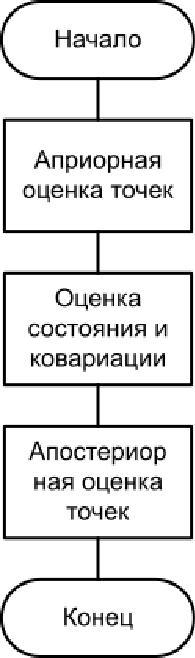
\includegraphics[height=10cm]{ukf_predict}}
\caption{Алгоритм шага предсказания UKF}
\label{fig:ukf_predict}
\end{figure}

На этапе предсказания UKF генерирует набор сигма-точек на основе текущей оценки состояния и ковариации, 
пропускает их через модель системы для прогнозирования следующего состояния и ковариации.
На этапе обновления, при поступлении измерений, сигма-точки пропускаются через модель измерений, после чего вычисляются среднее измерение, 
ковариация и коэффициент усиления Калмана, используемые для корректировки состояния и ковариации с учётом новых данных.
Этот подход позволяет UKF эффективно обрабатывать нелинейности и обеспечивать точную оценку состояния.

\FloatBarrier
\begin{figure}[H]
\centering
	\fbox{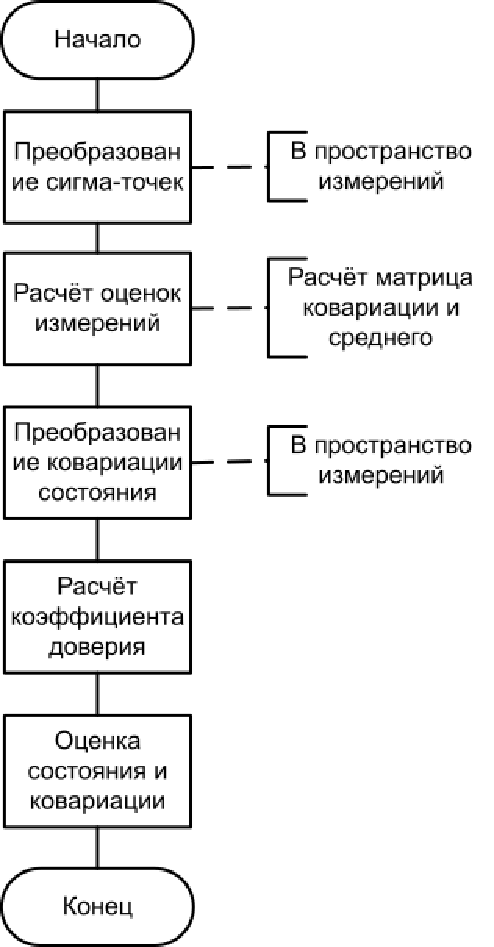
\includegraphics[height=12cm]{ukf_update}}
\caption{Алгоритм шага обновления UKF}
\label{fig:ukf_update}
\end{figure}

\subsubsection{События обновления состояния}

Данные от датчиков формируют события изменения состояния. 
Все события изменяют состояние системы в соответствии с алгоритмом обработки событий (см. рисунок \ref{fig:handle_kf_event})

\FloatBarrier
\begin{figure}[H]
\centering
	\fbox{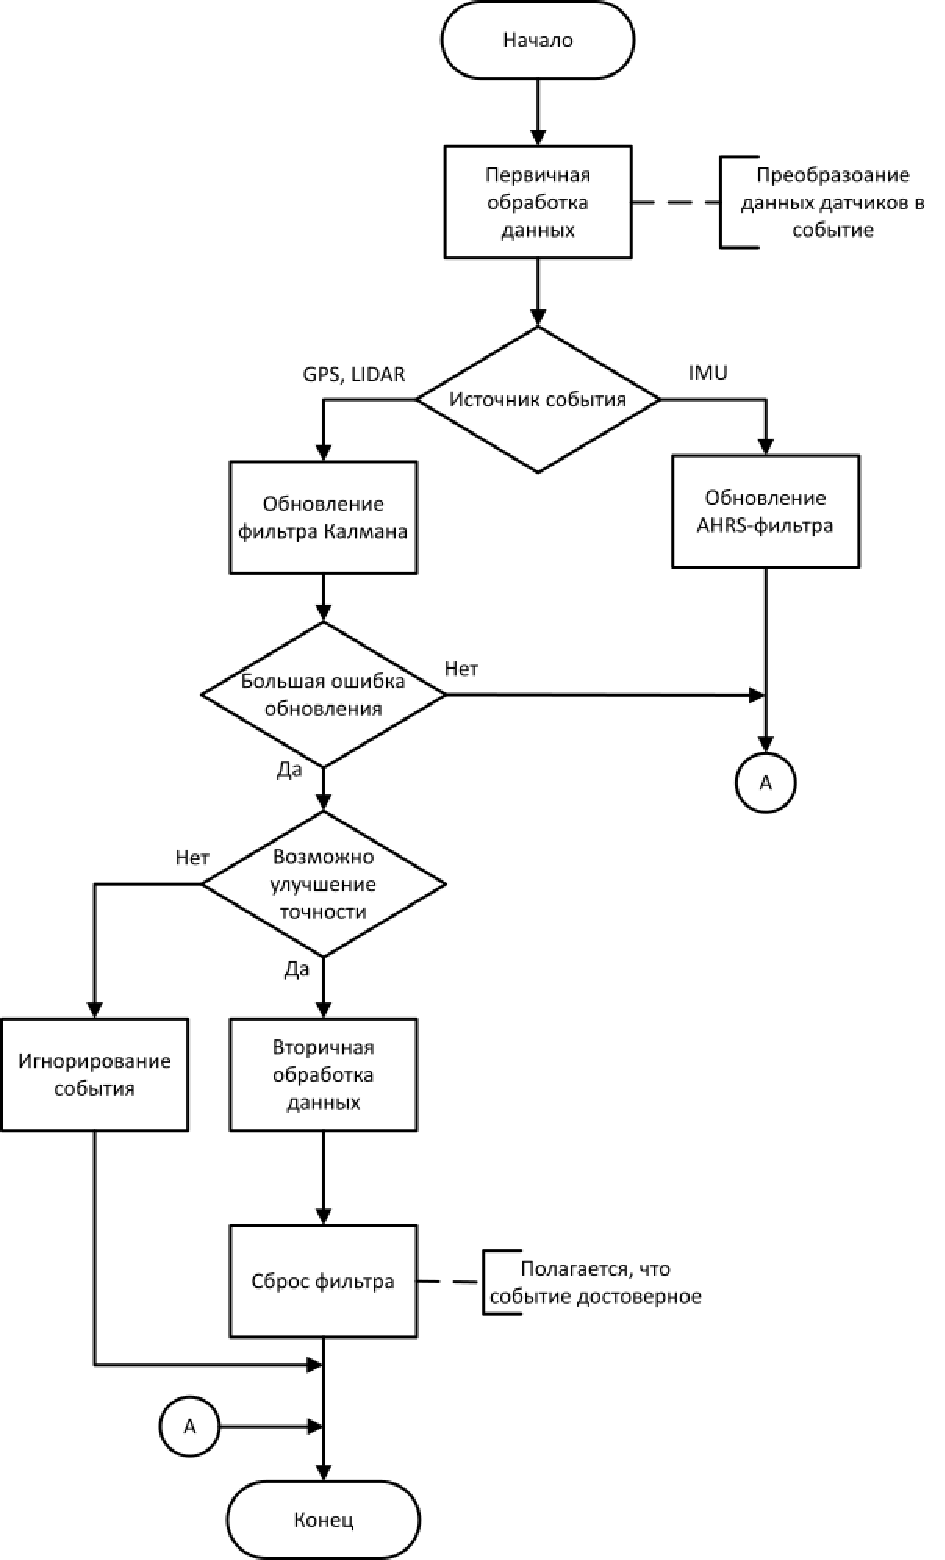
\includegraphics[height=12cm]{handle_event}}
\caption{Алгоритм обработки событий}
\label{fig:handle_kf_event}
\end{figure}


Обновление состояния в UKF выполняется только по позиционным событиям, 
которые происходят относительно редко, но обладают высокой точностью.
Позиционными событими являются содержат оценку координат робот в системе координат локальной карты робота ($x, y$) и
необязательную оценку ориентации робота в пространстве ($\theta$).
К таким событиям относятся результаты обработки данных от GPS и LIDAR.

Для обработки данных IMU используется фильтр Маджвика (см. подраздел \href{sec:ahrs}). Было принято решение использовать
отдельный фильтр для обработки данных IMU, а не обновлять вектор системы ${X}$,
по следующим причинам:
\begin{itemize}
	\item данные IMU измеряют только ориентацию, потому фильтр не сможет произвести коррекцию
	      всего вектора состояния во времени;
        \item данные от IMU приходят с гораздо большей частотой (1000 Hz), чем данные от LIDAR (10 Hz) или GPS (5 Hz).
\end{itemize}

Оценка ориентации с помощью фильтра Маджвика используется 
в процессе обработки данных LIDAR или GPS для формирования позиционных событий.

Таким образом, использованием фильтра Маджвика обеспечивает надежную и частую оценку ориентации, в то время как UKF использует редкие, но точные позиционные данные для коррекции полного вектора состояния.
Это повышает общую точность и устойчивость системы в условиях сложной динамики и возможных выбросов в измерениях.

\subsection{Очереди событий и очереди состояний}
\label{subsec:queues}

Каждое состояние системы ${X}_k$ и событие ${E}_k$ 
закреплено к моменту времени $t_k$. Каждое новое событие 
обновляет модель системы в сооветствие с алгоритмом применения события (см. рисунок \ref{fig:apply_kf_event})
\FloatBarrier
\begin{figure}[H]
\centering
	\fbox{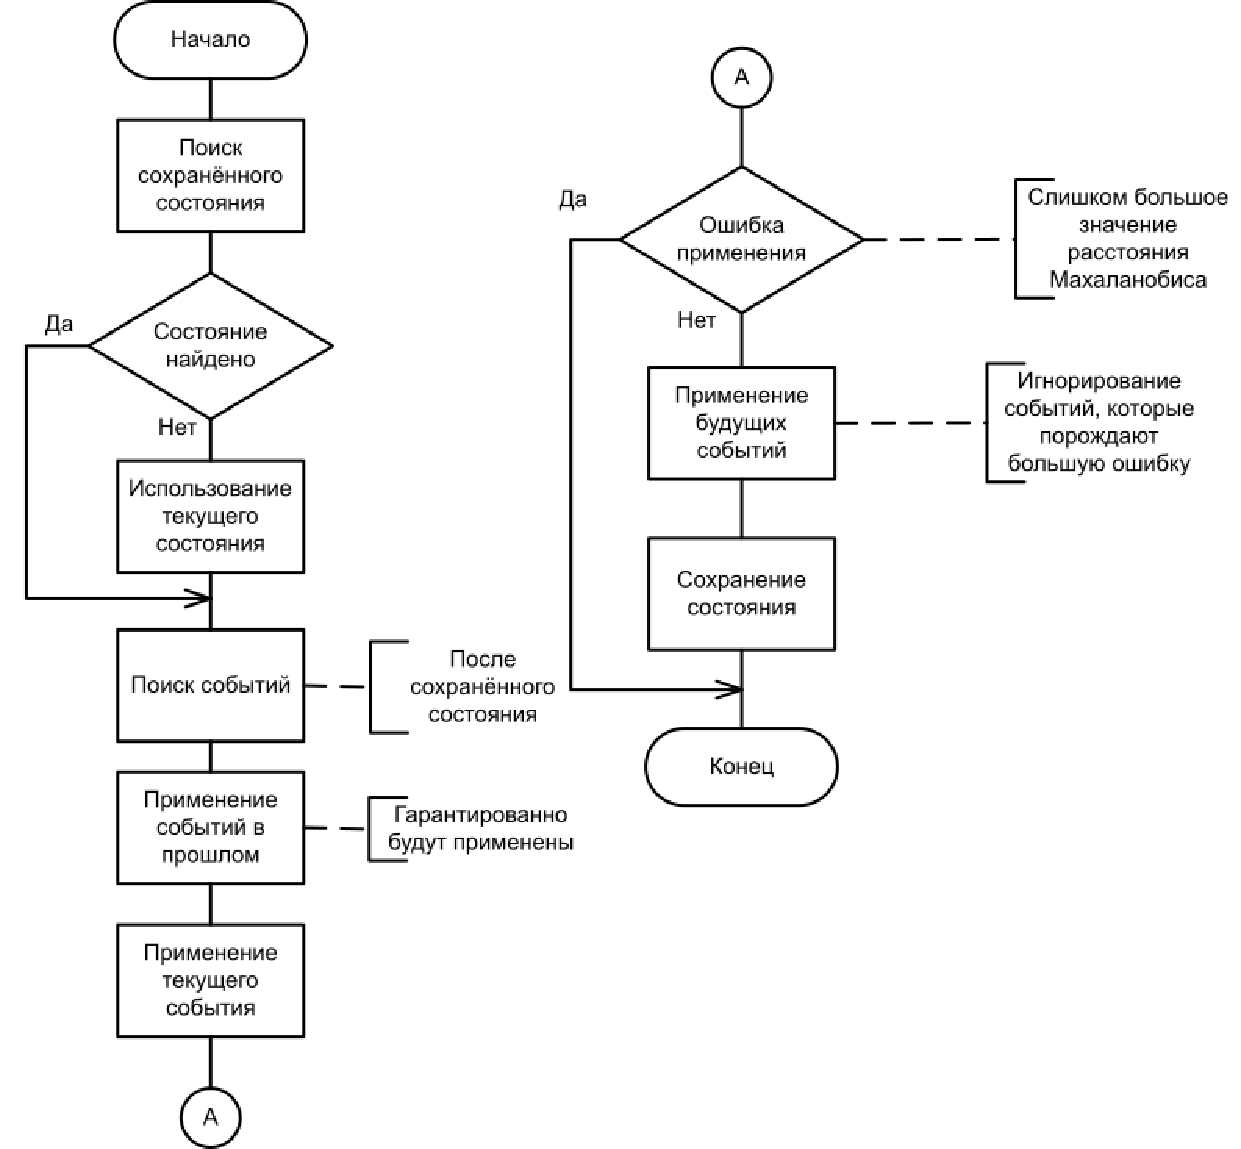
\includegraphics[height=12cm]{apply_event}}
\caption{Алгоритм применения события}
\label{fig:apply_kf_event}
\end{figure}

Для эффективной обработки данных и управления временной динамикой системы реализованы очереди состояний и событий.
Это позволяет синхронизировать данные от различных источников и корректно обновлять состояние системы в UKF.

\subsubsection{Очередь состояний}
\label{subsec:state_queue}

Очередь состояний представляет собой упорядоченный набор векторов состояния системы.
Основные характеристики очереди состояний:
\begin{itemize}
    \item каждое состояние в очереди соответствует определённому моменту времени, что позволяет отслеживать эволюцию системы и выполнять ретроспективные корректировки при получении новых данных;
    \item временные метки состояний используются для сопоставления с событиями, обеспечивая согласованность между предсказаниями и измерениями;
    \item при поступлении новых данных очередь состояний обновляется, добавляя новое состояние.
\end{itemize}

\subsubsection{Очередь событий}
\label{subsec:event_queue}

Очередь событий содержит результаты обработки данных от датчиков. Каждое из событие связано с моментом времени $t$.
События представляют собой позиционные данные, которые используются для коррекции состояния в UKF.
Основные характеристики очереди событий:
\begin{itemize}
    \item каждое событие имеет метку времени для определения положения относительно текущего момента времени;
    \item относительно события с временем $t_{\text{current}}$ события разделяются на события прошлого и события будущего;
    \item события прошлого используются для ретроспективной коррекции состояний, если данные поступили с задержкой или требуется уточнение предыдущих оценок;
    \item события будущего хранятся в очереди для обработки по мере продвижения текущего времени системы. Это позволяет системе быть готовой к асинхронным данных.
    \item очередь событий поддерживает асинхронное поступление данных от датчиков с разной частотой. 
\end{itemize}

\subsection{Планирование движения}

\subsubsection{Локальный планировщик}
В качестве локального планировщика используется DWA.
Целевая функция:
\begin{equation}
	G(v, \omega) = \sum_{i=1}^k w_i \cdot g_{i, \text{norm}}(v, \omega),
\end{equation}

\begin{explanationx}
	\item[где] $g_{i,\text{norm}}(v, \omega)$ -- значение $i$-й подцелевой функции;
	\item $w_i$ -- весовой коэффициент,
		настраиваемый для задания приоритетов;
	\item $k$ -- количество метрик.
\end{explanationx}

Для обеспечения сравнимости метрик,
имеющих разные единицы измерения и диапазоны,
значения подцелевых функций $g_i(v, \omega)$ нормализуются по всем возможным парам скоростей 
в динамическом окне $V_d$.
Нормализованное значение вычисляется как:
\begin{equation}
	g_{i, \text{norm}}(v, \omega) = \frac{g_i(v, \omega) - \min_{(v', \omega') \in V_d} g_i(v', \omega')}{\max_{(v', \omega') \in V_d} g_i(v', \omega') - \min_{(v', \omega') \in V_d} g_i(v', \omega')},
\end{equation}

\begin{explanationx}
	\item[где] $\min_{(v', \omega') \in V_d} g_i(v', \omega')$ --
минимальное значения $i$-й подцелевой функции среди всех пар $(v', \omega')$ в $V_d$.
	\item $\max_{(v', \omega') \in V_d} g_i(v', \omega')$ --
максимальное значения $i$-й подцелевой функции среди всех пар $(v', \omega')$ в $V_d$.
\end{explanationx}

Нормализация приводит значения к диапазону $[0, 1]$, что позволяет весам $w_i$ эффективно управлять
приоритетами метрик и обеспечивает сбалансированную оценку траекторий.

Для каждой пары скоростей предлагается построение уникальной траектории.
Оценка происходит не столько по значениями скорости, сколько по траекториям, которые скорости генерируют.
В качестве метрик предлагается использовать:

    1 Метрика близости к цели -- чем ближе конечная точка траектория к цели, тем траектория приоритетнее.

    2 Метрика близости к глобальной траектории -- чем ближе форма траектории к прямолинейной форме траектории, тем траектория приоритетнее.  

    3 Метрика избегания препятствий -- приоритет отдаётся тем траектории, которые проходят дальше от препятствий.

    4 Метрика колебательных движений -- предотвращает резкие (осциллирующие) изменения скоростей для обеспечения плавности и зацикливания.

    5 Выравнивание по целевой ориентаци -- инимизирует отклонение ориентации робота от желаемого угла в целевой точке.

    6 Метрика коллизий -- отклоняет все траектории, в которых обнаружены столкновения с объектами препятствий.

% \subsubsection{Применение}

% \subsubsection{Глобальный планировщик}

\subsection{Взаимодействие с периферией}


В процессе разработки программного обеспечения для автономной навигации
мобильных платформ одной из ключевых задач стало обеспечение гибкого и надёжного
взаимодействия с периферийными устройствами, такими как датчики, камеры и
лидары. После анализа различных подходов было принято решение реализовать это
взаимодействие с использованием стека протоколов TCP/IP. Такой выбор обусловлен
универсальностью и стандартизацией данного протокола, который широко применяется
в сетевых технологиях и позволяет организовать стабильное соединение между
компонентами системы. Это решение обеспечивает возможность передачи данных в
реальном времени, что критически важно для задач управления и обработки
информации в динамичной среде.

Использование TCP/IP стека предоставляет значительное преимущество в виде
модульности и расширяемости системы. Благодаря этому подходу стало возможным
подключение различных датчиков к программе непосредственно во время её работы,
без необходимости останавливать или перезапускать систему. Например, если в
процессе эксплуатации мобильной платформы потребуется добавить новый лидар или
ультразвуковой датчик, это можно сделать "на лету", что существенно повышает
адаптивность системы к изменяющимся условиям или требованиям задачи. Такая
гибкость особенно ценна в экспериментальных или полевых условиях, где заранее
предусмотреть все сценарии использования невозможно.

Реализация взаимодействия через TCP/IP также упрощает интеграцию с современными
технологиями и стандартами, используемыми в робототехнике. Например, многие
устройства уже имеют встроенную поддержку сетевых протоколов, что позволяет
избежать разработки сложных проприетарных интерфейсов для каждого типа
периферии. Кроме того, TCP/IP обеспечивает надёжную передачу данных с механизмом
проверки ошибок, что снижает риск потери критически важной информации от
датчиков. Это особенно актуально для автономных систем, где точность и
своевременность получения данных напрямую влияют на качество навигации и
принятия решений.

% \subsection{Разработка архитектуры модуля \todo{MotionEstimation}}
%
% \todo{Схема для motionEstimation}
%
% \subsection{Разработка архитектуры модуля \todo{BigMap}}
%
% \subsection{Разработка архитектуры модуля \todo{ScanMatching}}
%
% \subsection{Разработка архитектуры модуля \todo{TODO}}
